\documentclass[
10pt, % Main document font size
a4paper, % Paper type, use 'letterpaper' for US Letter paper
oneside, % One page layout (no page indentation)
%twoside, % Two page layout (page indentation for binding and different headers)
headinclude,footinclude, % Extra spacing for the header and footer
BCOR5mm, % Binding correction
]{scrartcl}

\usepackage{graphicx}
\usepackage{tikz-er2}
\usepackage[colorlinks, urlcolor=blue, linkcolor=black]{hyperref}

\title{Tp Sistema de Logistica}
\author{Matias M. Marceca}
\date{}

\begin{document}

\maketitle

\tableofcontents

%\pagebreak

\section {Analisis del Mercado Consumidor}
\subsection {Perfil y Comportamiento del consumidor}
  El surgimiento de la necesidad de logistica para el transporte de
  productos o individuos, se origino en la Ingenieria Militar.
  El objetivo fue trasladar Miles de soldados al mismo tiempo utilizando
  varios y variados metodos evitando que el enemigo note su transporte
  y llegada al objetivo.
  Para llevar a cabo tal plan, se originan los planes de transportes.
  \newline\newline
  Actualmente las Empresas de Logistica tienen como objetivo, planificar el
  traslado de Personas, Productos, Materia Prima, etc, de un lugar a otro.
  Para ello se requiere de una gran infraestructura para poder satisfacer
  varias etapas que cumplen con el objetivo planteado.
  \newline\newline
  Algunas etapas son :
  \begin{itemize}
    \item  Analisis de Trayecto de Mercaderia
    \item  Distribucion de Productos por transporte
    \item  Administracion de Stock de Productos
  \end{itemize}


\subsection {Alcance Estimado}
  Actualmente el Sistema estara al alcance de Empresas de Transporte terrestre
  para luego poder expandirlo a otros tipos de carga gracias a su facilidad de
  incorporacion de paquetes de modulos utilizados en la estrategia de venta.

 \textbf{Servicios que ofrecen nuestros clientes:}
 \begin{flushleft}
     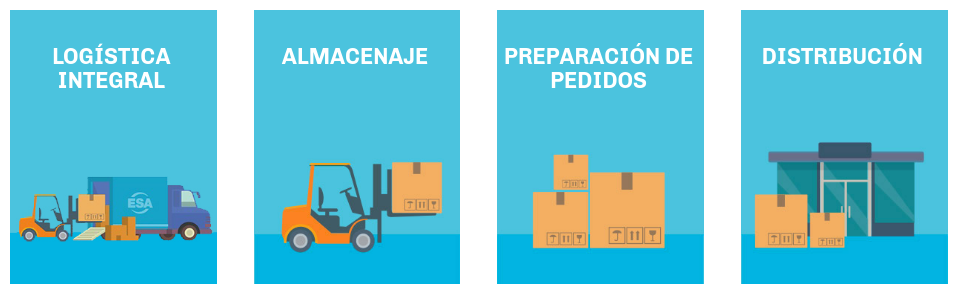
\includegraphics[width=14cm, keepaspectratio]{images/services.png}
 \end{flushleft}
  \begin{itemize}
    \item \textit{Imagen de la empresa :}
      \href{http://www.esalogistica.com.ar/index.html#quehacemos} {Link}
  \end{itemize}
  \begin{quotation}
    Actualmente, nuestro sistema cuenta con cada uno de los modulos requeridos
    por los clientes promedios para satisfacer cada una de sus necesidades.
  \end{quotation}
 \textbf{Que transportan:}
 \begin{flushleft}
     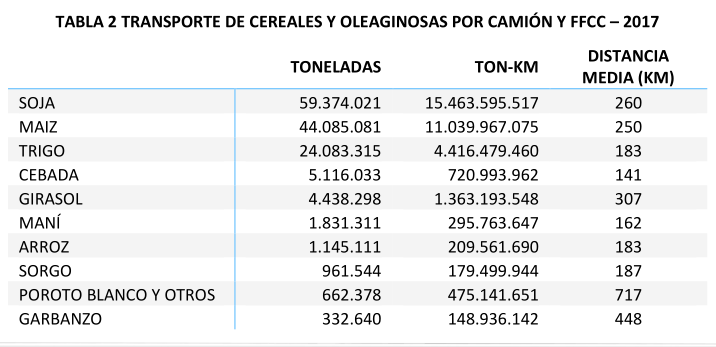
\includegraphics[width=10cm, keepaspectratio]{images/loads.png}
 \end{flushleft}
  \begin{itemize}
    \item \textit{Link al PDF del Gobierno de la Ciudad :}
      \href{https://www.argentina.gob.ar/sites/default/files/transporte_terrestre_de_cereales_y_oleaginosas_2017_v1.pdf} {Link}
  \end{itemize}
  \begin{quotation}
    El volumen de mercaderia que transportan nuestros clientes es tan
    importante para ellos como para nosotros asegurar la fidelidad de las
    cantidades ingresadas para una mayor seguridad a la hora de generar
    reportes mensuales con estadisticas de los ingresos netamente generados.
  \end{quotation}
 \textbf{Ciudades Recorridas:}
 \begin{flushleft}
     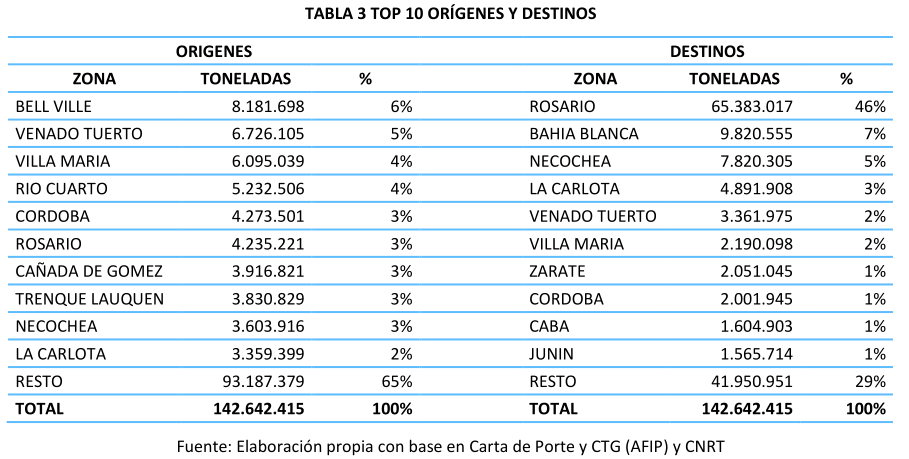
\includegraphics[width=12cm, keepaspectratio]{images/cities.png}
     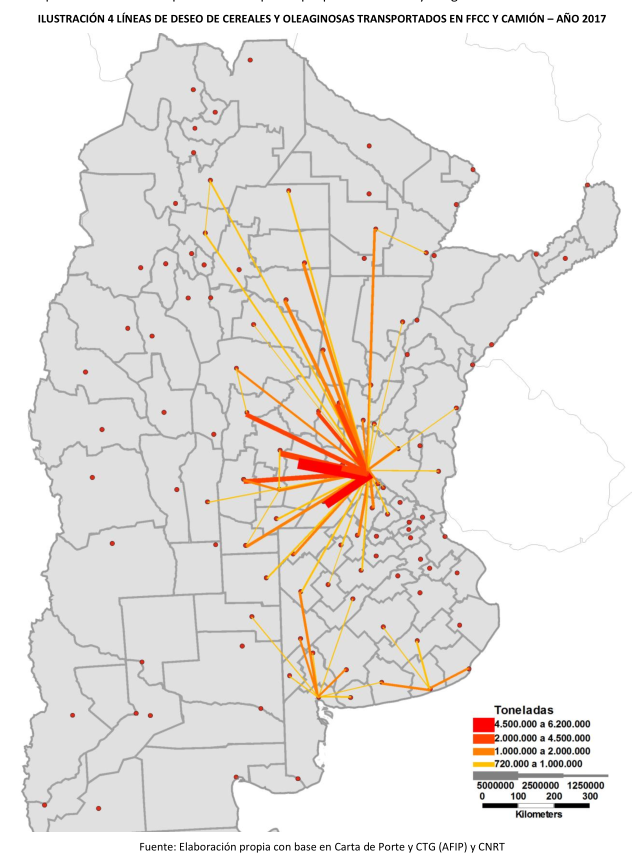
\includegraphics[width=12cm, keepaspectratio]{images/country_map.png}
 \end{flushleft}
  \begin{itemize}
    \item \textit{Link al PDF del Gobierno de la Ciudad :}
      \href{https://www.argentina.gob.ar/sites/default/files/transporte_terrestre_de_cereales_y_oleaginosas_2017_v1.pdf} {Link}
  \end{itemize}
  \begin{quotation}
    La administracion del almacenaje de los productos son tan importantes como
    saber la posicion actual a medida que son transportados, ya que pueden
    surgir retrasos en el envio por motivos varios. En esos casos es necesario
    contar con rutas y estrategias alternativas para solventar el problema.
  \end{quotation}
 \textbf{Volumen de Cargas Anuales:}
 \begin{flushleft}
     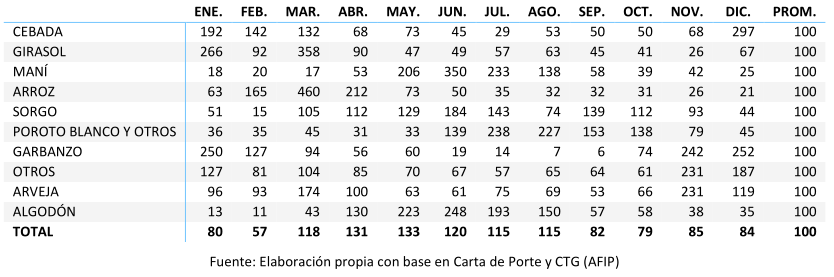
\includegraphics[width=14cm, keepaspectratio]{images/annual_work_i.png}
     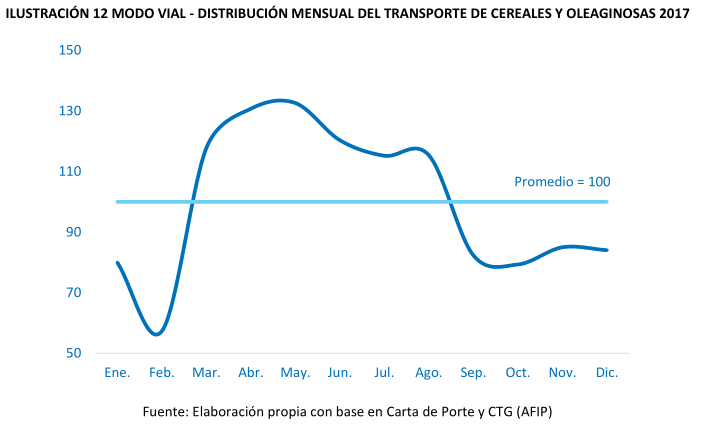
\includegraphics[width=14cm, keepaspectratio]{images/annual_work_ii.png}
 \end{flushleft}
  \begin{itemize}
    \item \textit{Link al PDF del Gobierno de la Ciudad :}
      \href{https://www.argentina.gob.ar/sites/default/files/transporte_terrestre_de_cereales_y_oleaginosas_2017_v1.pdf} {Link}
  \end{itemize}
  \begin{quotation}
    Con el volumen de Carga manejado anualmente, se ve la importancia de una
    buena administracion y seguridad de compra por parte del cliente al ver
    que puede acotar tiempos administrativos y utilizarlo en la busqueda de
    nuevas oportunidades o buscar nuevos horizontes.
  \end{quotation}


%\section {Principales Competencias}
% \begin{flushleft}
%     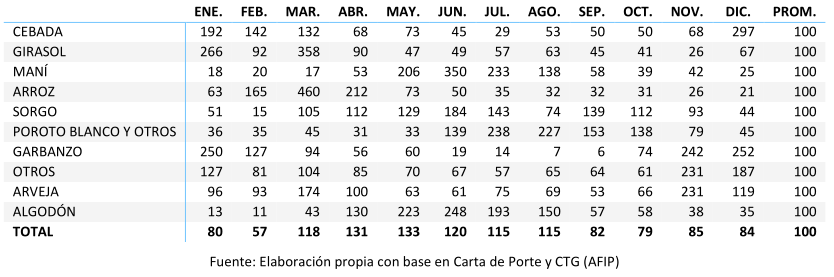
\includegraphics[width=17cm, keepaspectratio]{images/annual_work_i.png}
%     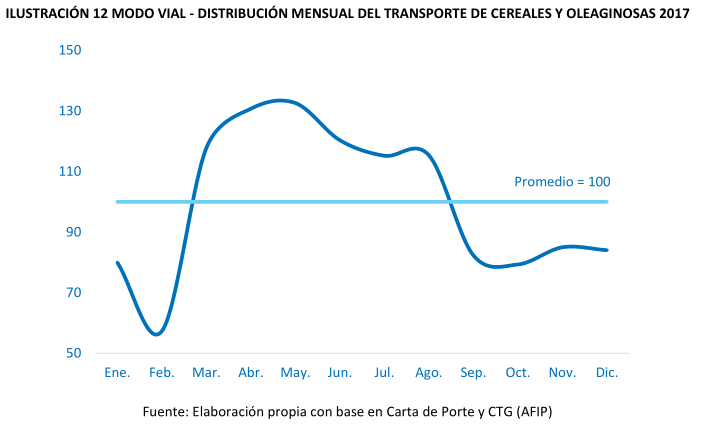
\includegraphics[width=17cm, keepaspectratio]{images/annual_work_ii.png}
% \end{flushleft}

\end{document}
